\section{Overview}

We introduce a general framework to design dynamic controllers using
high-level, human-readable instructions (Figure
\ref{fig:parkour_overview}). The iterative process begins with an input
controller. We view the initial controller as a blackbox because our
algorithm does not interact with its internal implementation. For all
our experiments, we used a simple pose-tracking controller with 4 to 6
keyframes. During training, the initial controller is improved
iteratively through alternating stages of \textit{coaching} and
\textit{practicing}. The output is a new controller that meets the
requirements of the user. Once a controller is developed, we can
generalize it by parameterization or concatenation for new situations.

\begin{figure}[ht]
\center
  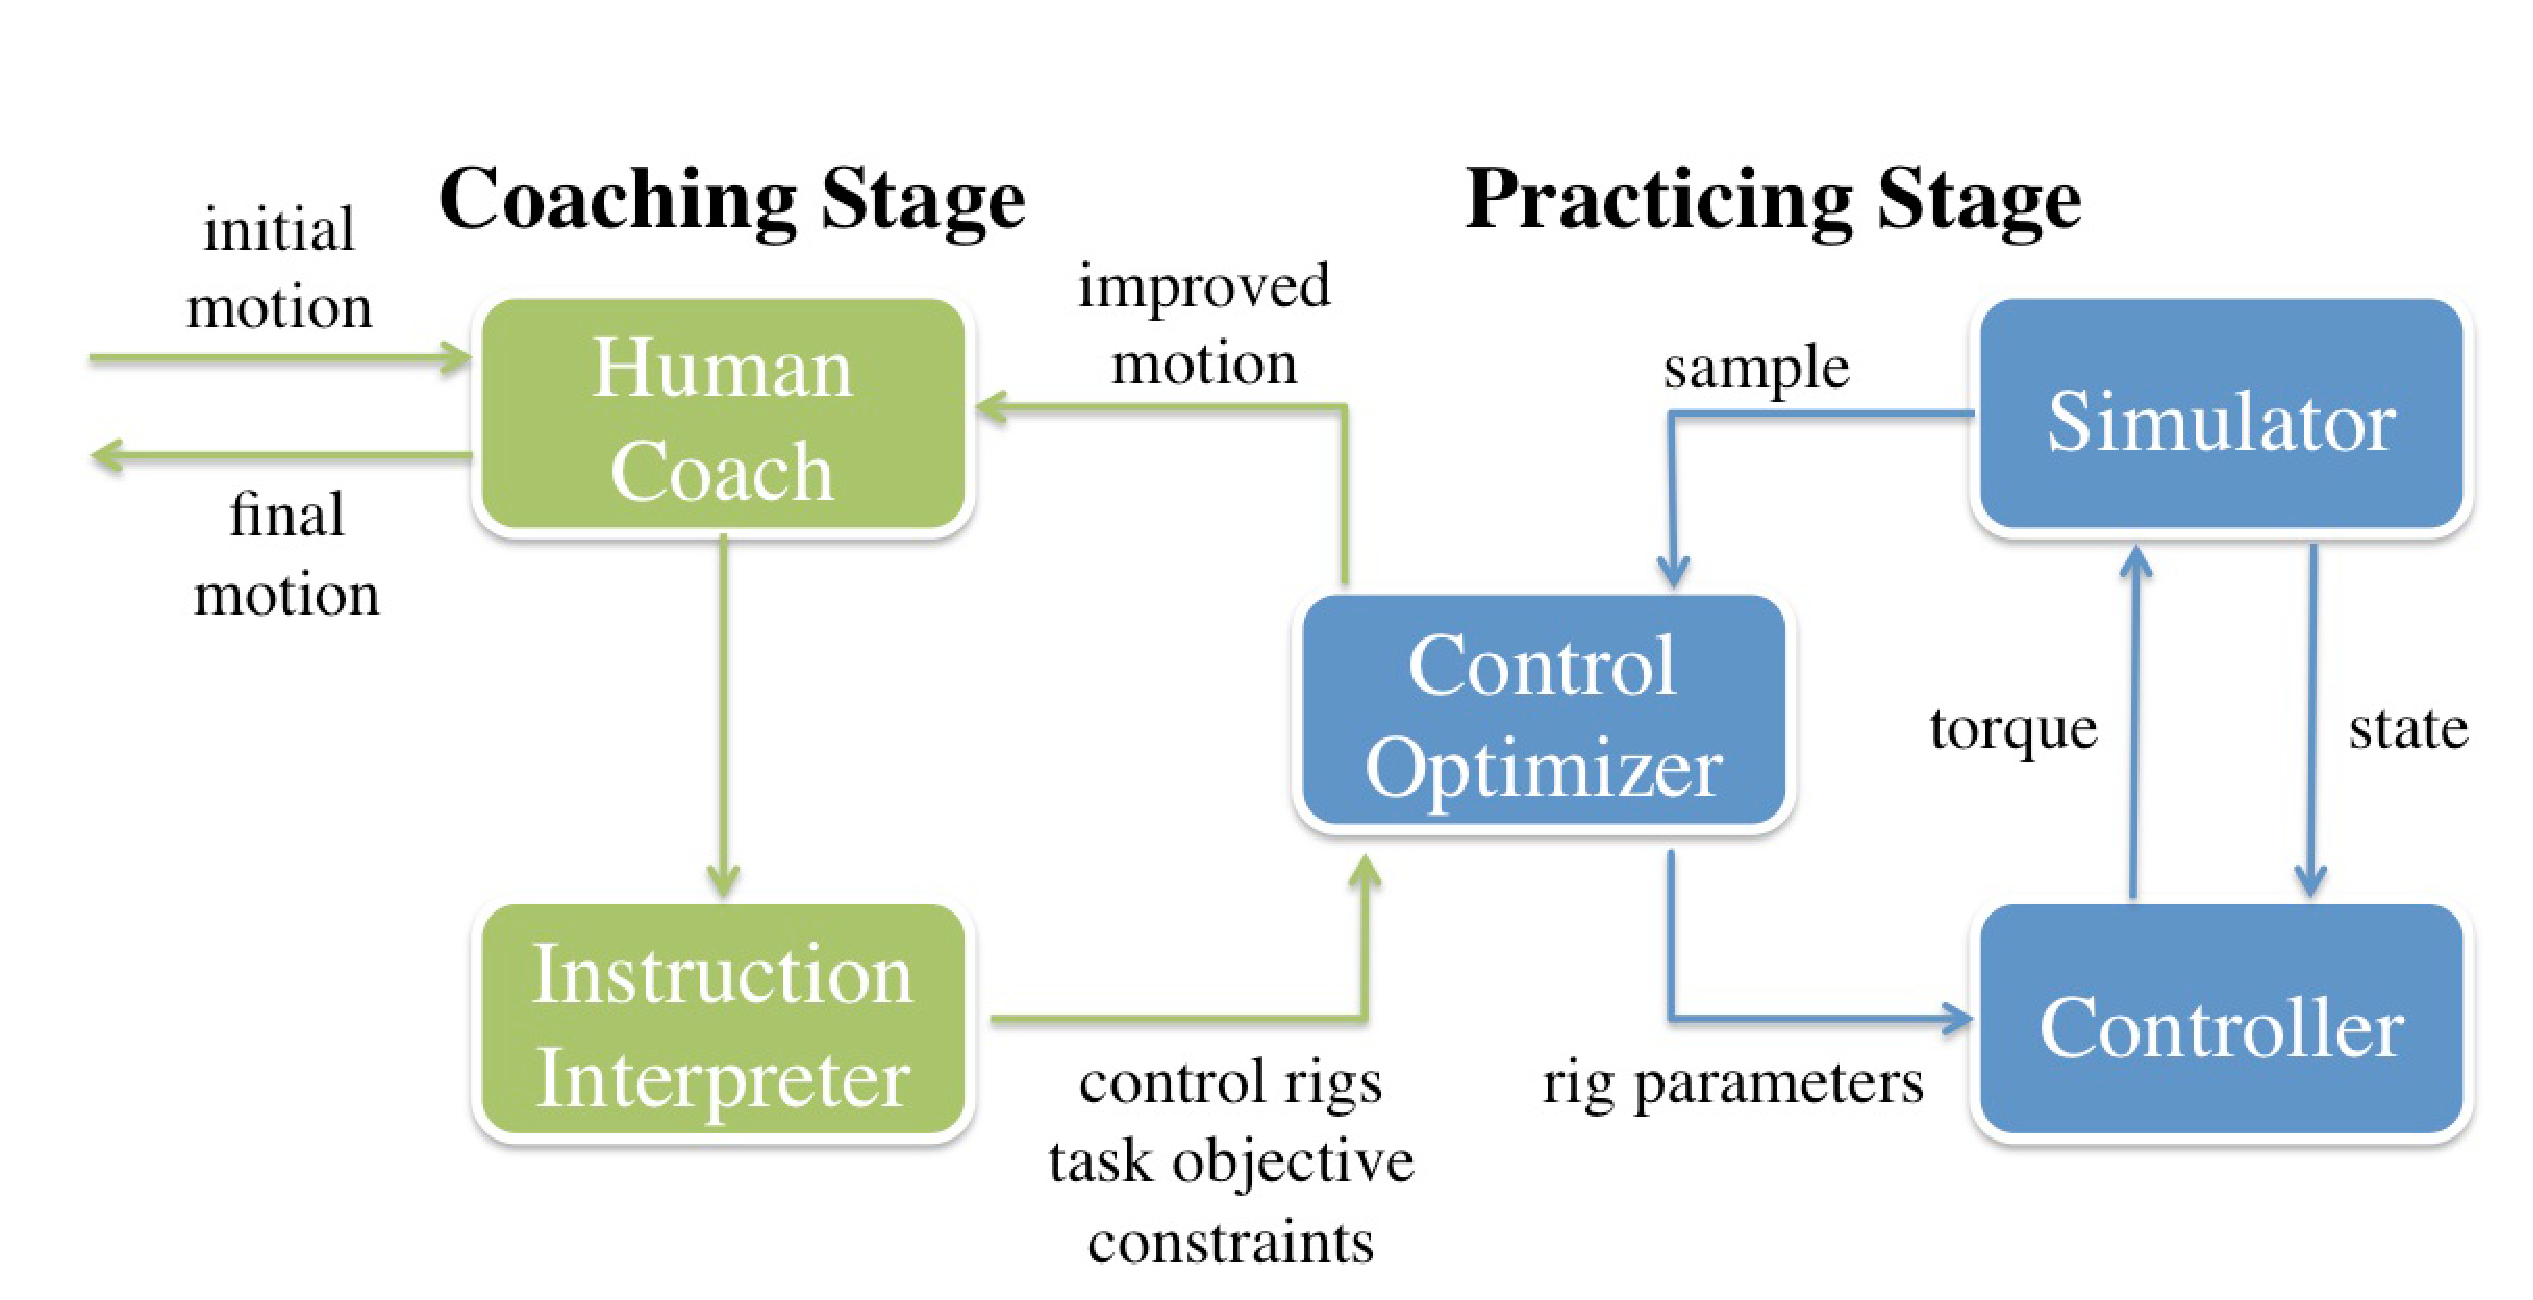
\includegraphics[width=4.2in]{images/diagram}
  \caption{
    Overview diagram. 
  }
  \label{fig:parkour_overview}
\end{figure}

During each coaching stage, the user provides high-level instructions
to correct undesired behaviors, change task objectives, or add
different styles to the motion. According to the type of the
instructions, the \textit{instruction interpreter} automatically selects
the appropriate control rigs, and modifies constraints or the
objective function for the optimization. 

During each practicing stage, the \textit{control optimizer} searches
for control rig parameters using our new algorithm, Covariance Matrix
Adaptation with Classification (CMA-C). The control optimizer uses the
current estimate of rig parameters to generate motion samples. A
controller can be represented as a function $g$, which takes the
current state $\vc{q}_t$ as input and generates torque $\tau_t$. In
addition, we denote $s$ as a function that simulates the motion from a
given state under a given controller, and outputs the final state
$\vc{q}_f$ of the simulation.
\begin{equation}
  \vc{q}_f = s(\vc{q}_t, g)
\end{equation}

